\documentclass[letterpaper,14pt,titlepage,fleqn]{article}

\setlength{\mathindent}{1cm}

\usepackage{graphicx}                                        

\usepackage{amssymb}                                         
\usepackage{amsmath}                                         
\usepackage{amsthm}                                          

\usepackage{alltt}                                           
\usepackage{float}
\usepackage{color}

\usepackage{url}

\usepackage{balance}
\usepackage[TABBOTCAP, tight]{subfigure}
\usepackage{enumitem}

\usepackage{pstricks, pst-node}

\usepackage{cite}
\usepackage{indentfirst}
\usepackage{listings}

% the following sets the geometry of the page
\usepackage{geometry}
\geometry{textheight=9in, textwidth=6.5in}

% random comment

\newcommand{\cred}[1]{{\color{red}#1}}
\newcommand{\cblue}[1]{{\color{blue}#1}}

\usepackage{hyperref}

\usepackage{textcomp}
\usepackage{listings}

\def\name{Haoxiang Wang; Student ID: 932359049}

%% The following metadata will show up in the PDF properties
\hypersetup{
  colorlinks = true,
  urlcolor = black,
  pdfauthor = {\name},
  pdfkeywords = {CS557 Project 5},
  pdftitle = {Project \#6: Deer Poster},
  pdfsubject = {Project \#6: Deer Poster},
  pdfpagemode = UseNone
}

\parindent = 0.0 in
\parskip = 0.2 in

\author{\name}
\title{Project \#6: Deer Poster}

\begin{document}
\maketitle

This project is the Sixth project I have done in this class, and it is a really open project. We are required to put a deer in a scene and make it looks cool. I was confused by the definition of ``cool'' and how to make my scene looks cool. The whole project only takes me a few hours to implement but takes me another several hours to figure out what should I implement. The results images and the explanation of how code works will be described in the after section. 

\section{Source Listing}
In this project, nine files are necessary. They are files handle the cube-mapping, files handle deer patterns, the deer object, and the textures. The specific filenames and usages are listed below.

deer.glib --- Handle the user interface and object\\
deer.vert --- Handle the vertex shader\\
deer.frag --- Handle the fragment shader\\
deer.obj --- Provide deer object\\
texture.vert --- Handle cube-mapping\\
texture.frag --- Handle cube-mapping\\
lt1.bmp, lt2.bmp, lt3.bmp --- Cube-mapping textures

\section{Result Images and Explanation}
My ``cool'' scene would be a deer covered by lightning coming through a lightning hole in the lightning cloud. To implement it, I used cube-mapping to create the environment around the deer, noise and smoothpulse to create the pattern on the deer's body, non-linear displacement to ``shrink'' the deer's body, and a fake silhouette to impelment shinny lightning covering deer's body. All features are controled by sliders in order to adjust for the best looking scene. The following image shows the origin look of the scene when the .glib file is loaded.
\begin{center}
	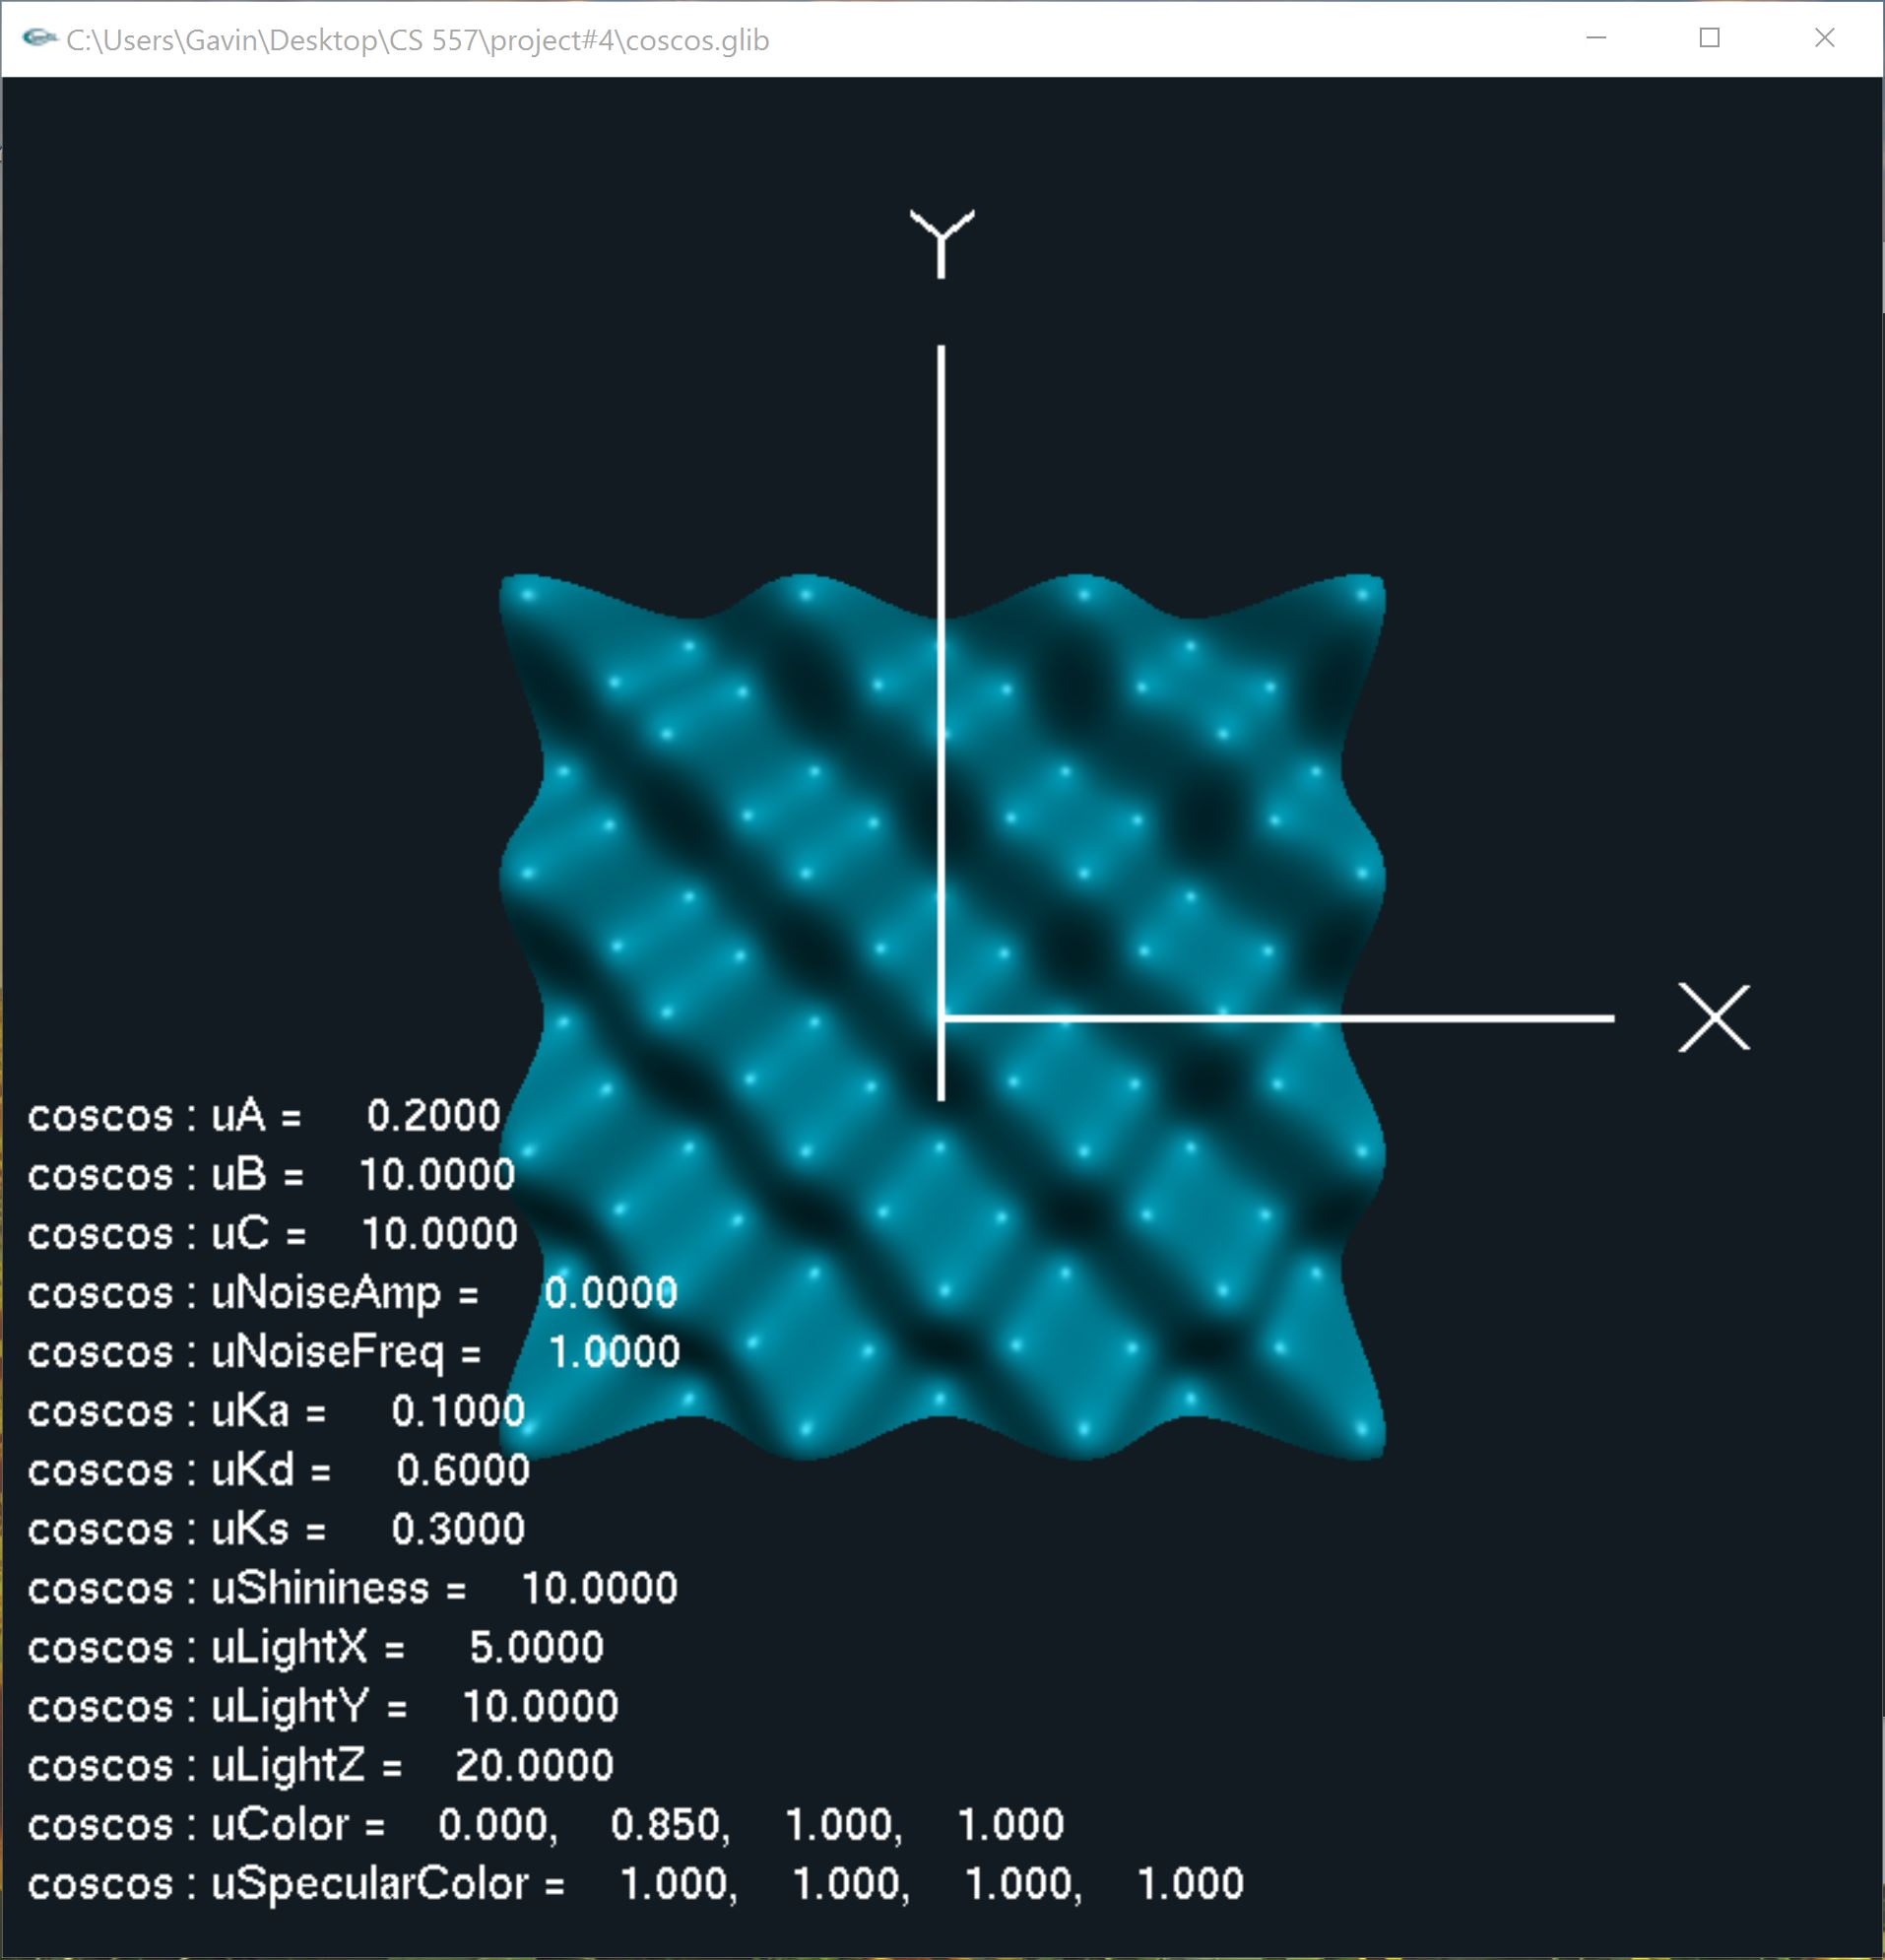
\includegraphics[width=3in]{origin.jpg}
\end{center}
As it mentioned in the previous section, this project contains several parts of implementation. The first part I would like to introduce is the non-linear displacement. It's located in the vertex shader. By applying the following euqtions to the vertexes' y and z coordinates, I kind of implemented a ``shrink'' effect to the part, which is the part in the positive x range, of the deer's body. The effect is shown in the following image.\\
The equations are: \\
$position.y = position.y*cos(PI/2*position.x/10);$\\
$position.z = position.z*cos(PI/2*position.x/10);$
\begin{center}
	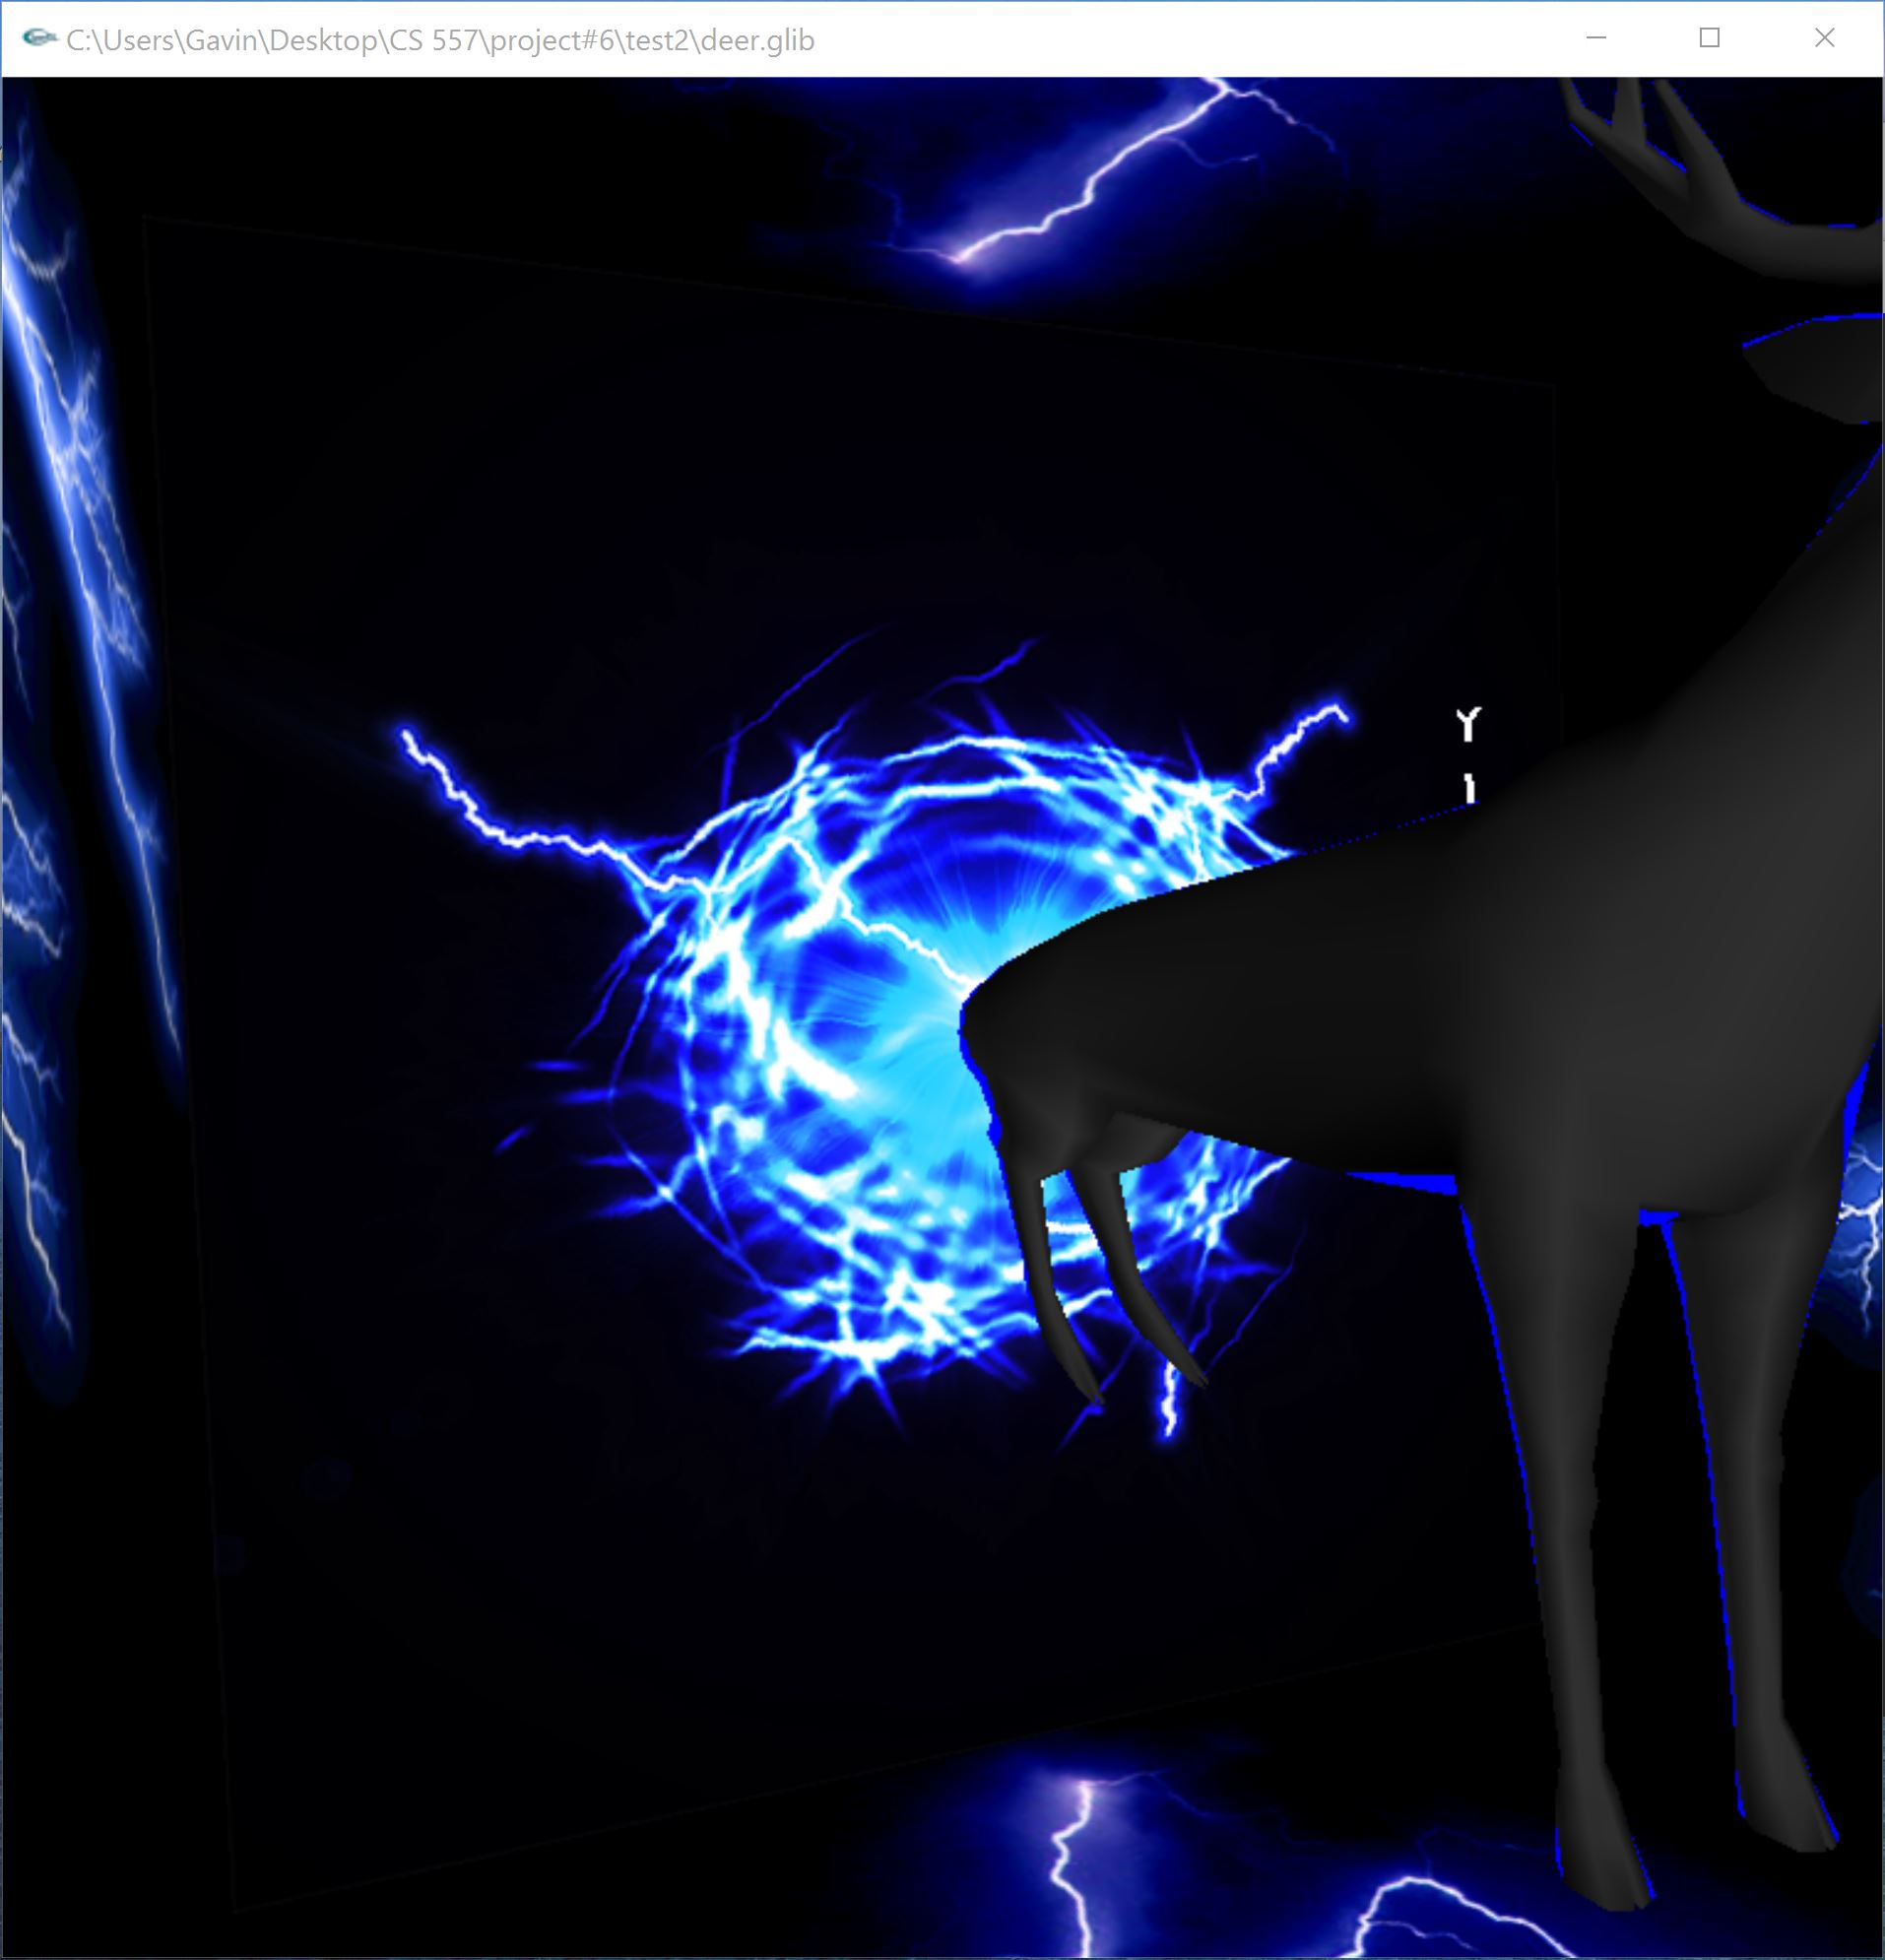
\includegraphics[width=2.9in]{shrink.jpg}
\end{center}
The second part is the implementation of the lightning pattern on the deer's body. It's implemented by applying noise and tolerance to several cyan-blue stripes. The stripes is created by the smoothpulse, which is two smoothsteps applied subtraction. By playing with the noise amplitude, frequency, the number and width of stripes, and the tolerance, a good-looking lightning pattern can be created. The following two images show the steps creating the pattern. The first one shows the original stripes, and the second one shows a complete pattern.
 \begin{center}
 	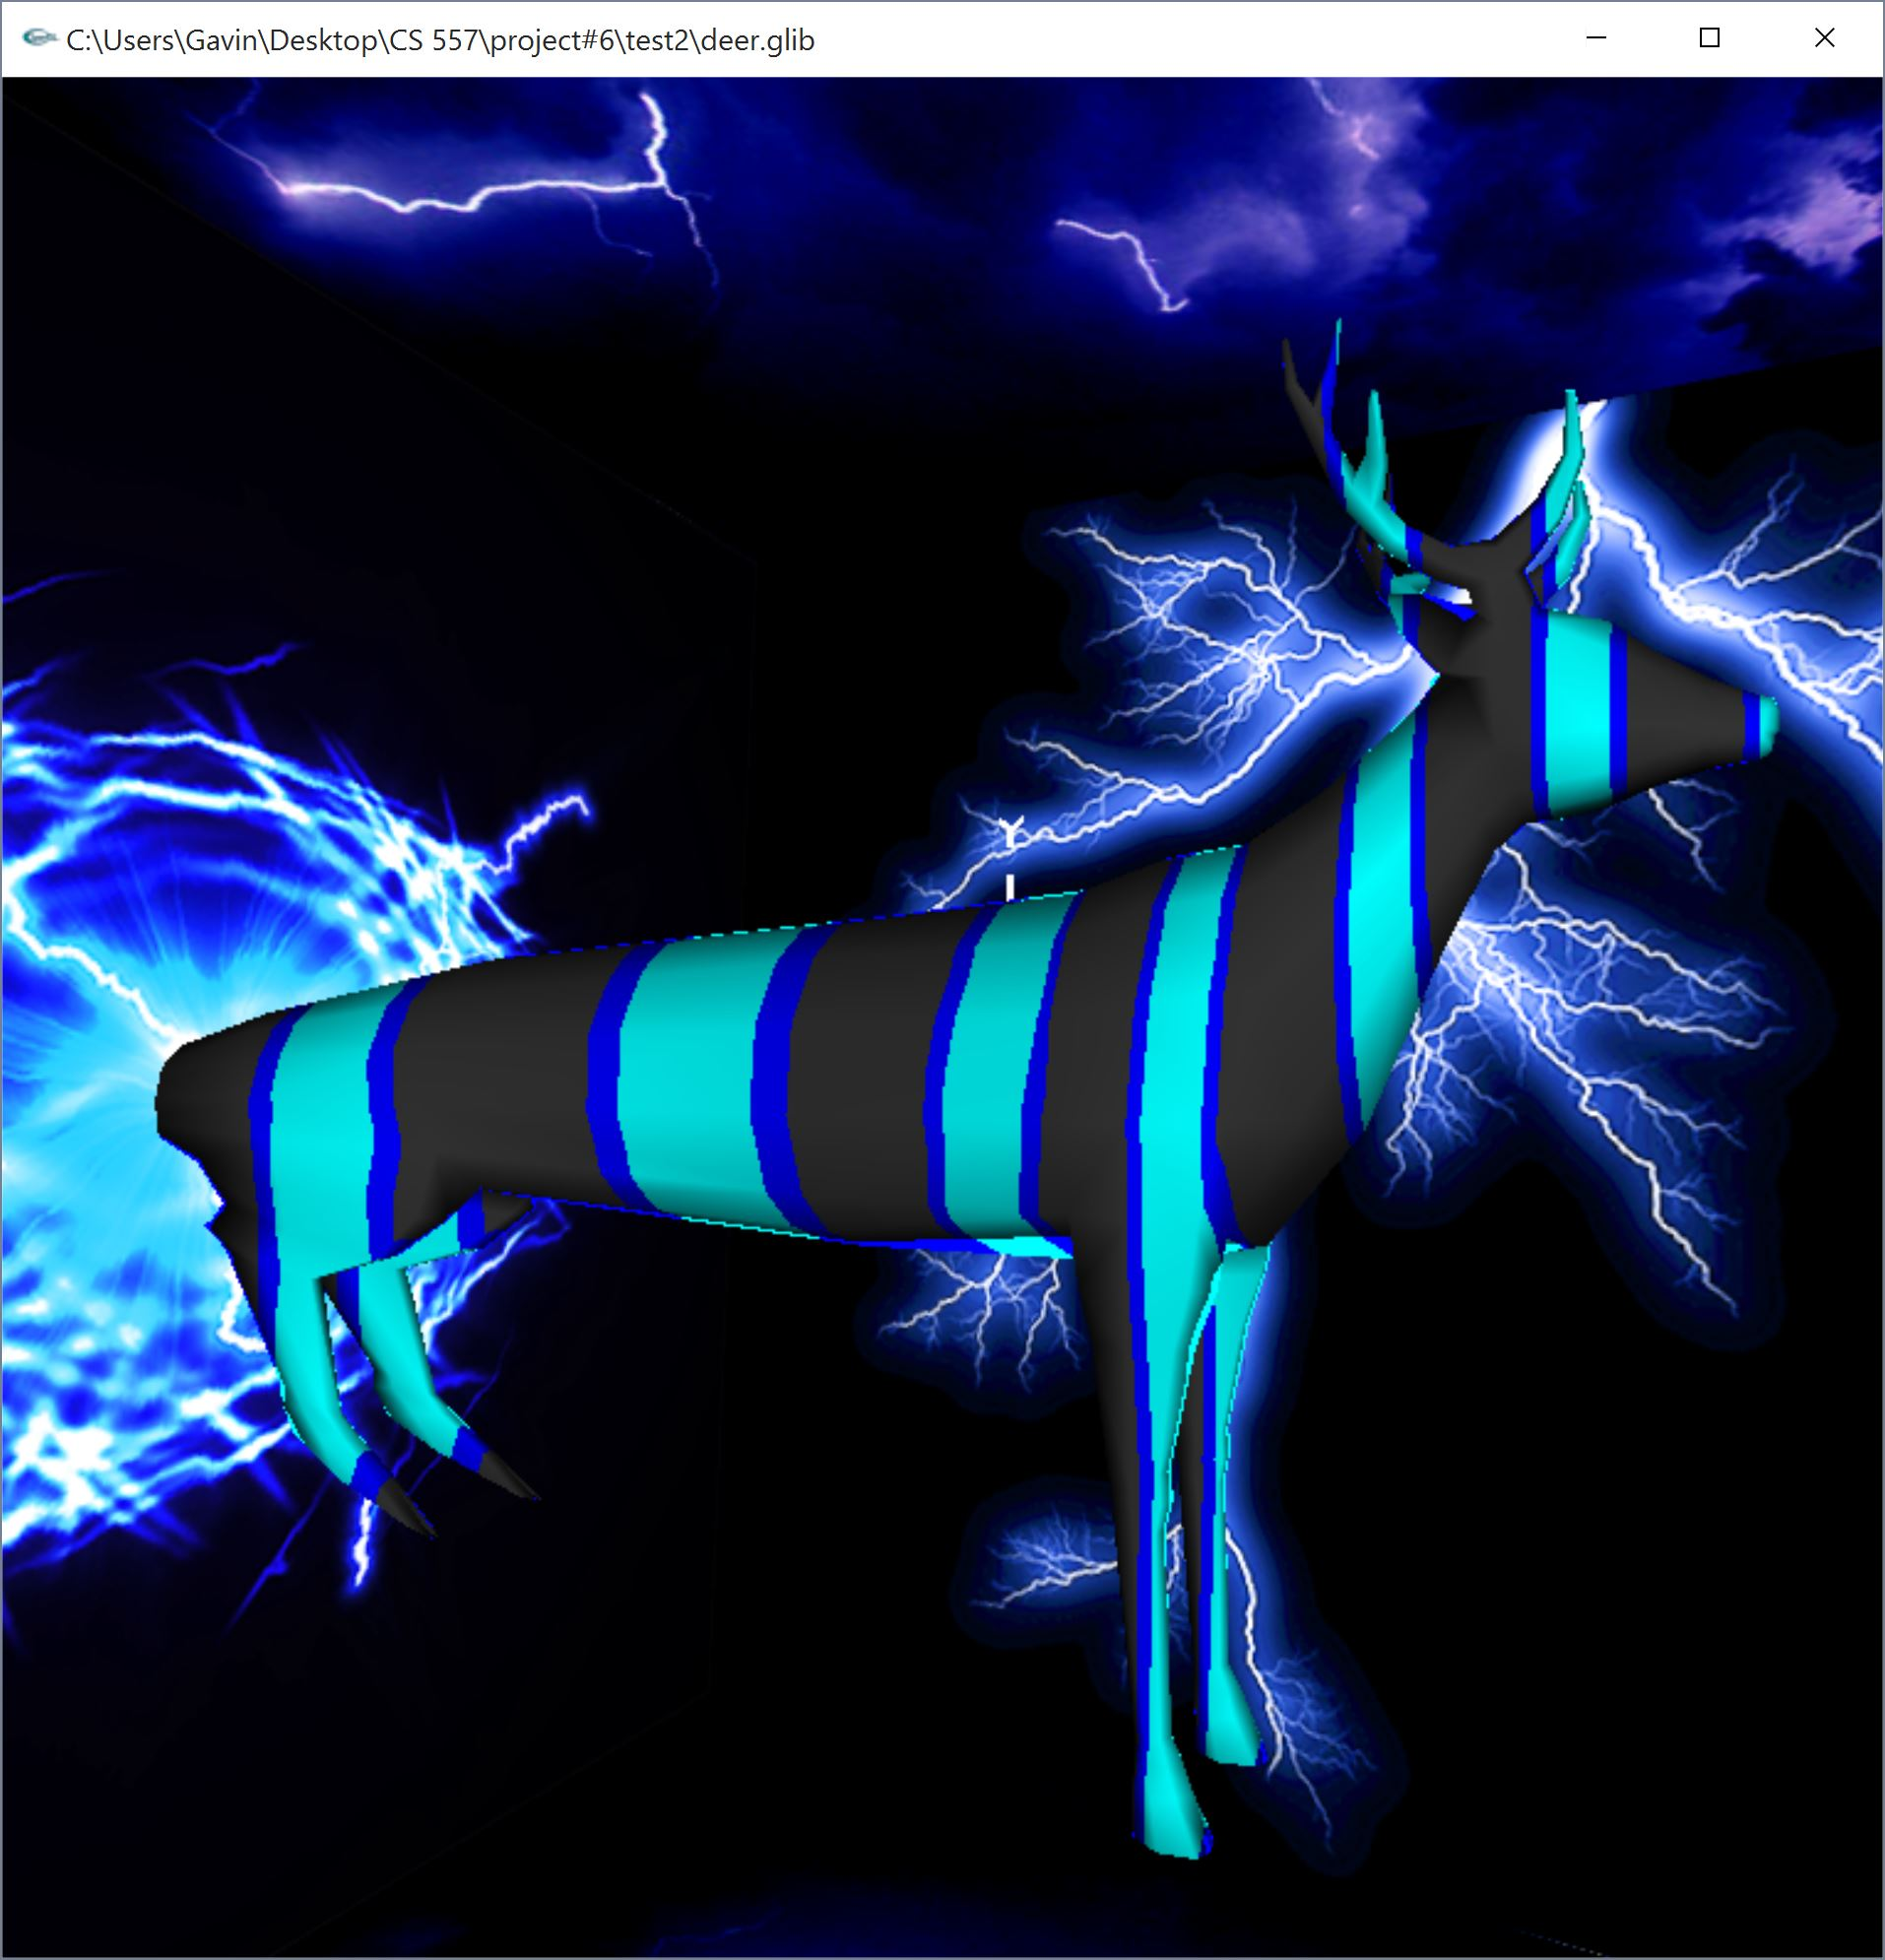
\includegraphics[width=2.8in]{strip.jpg}
 	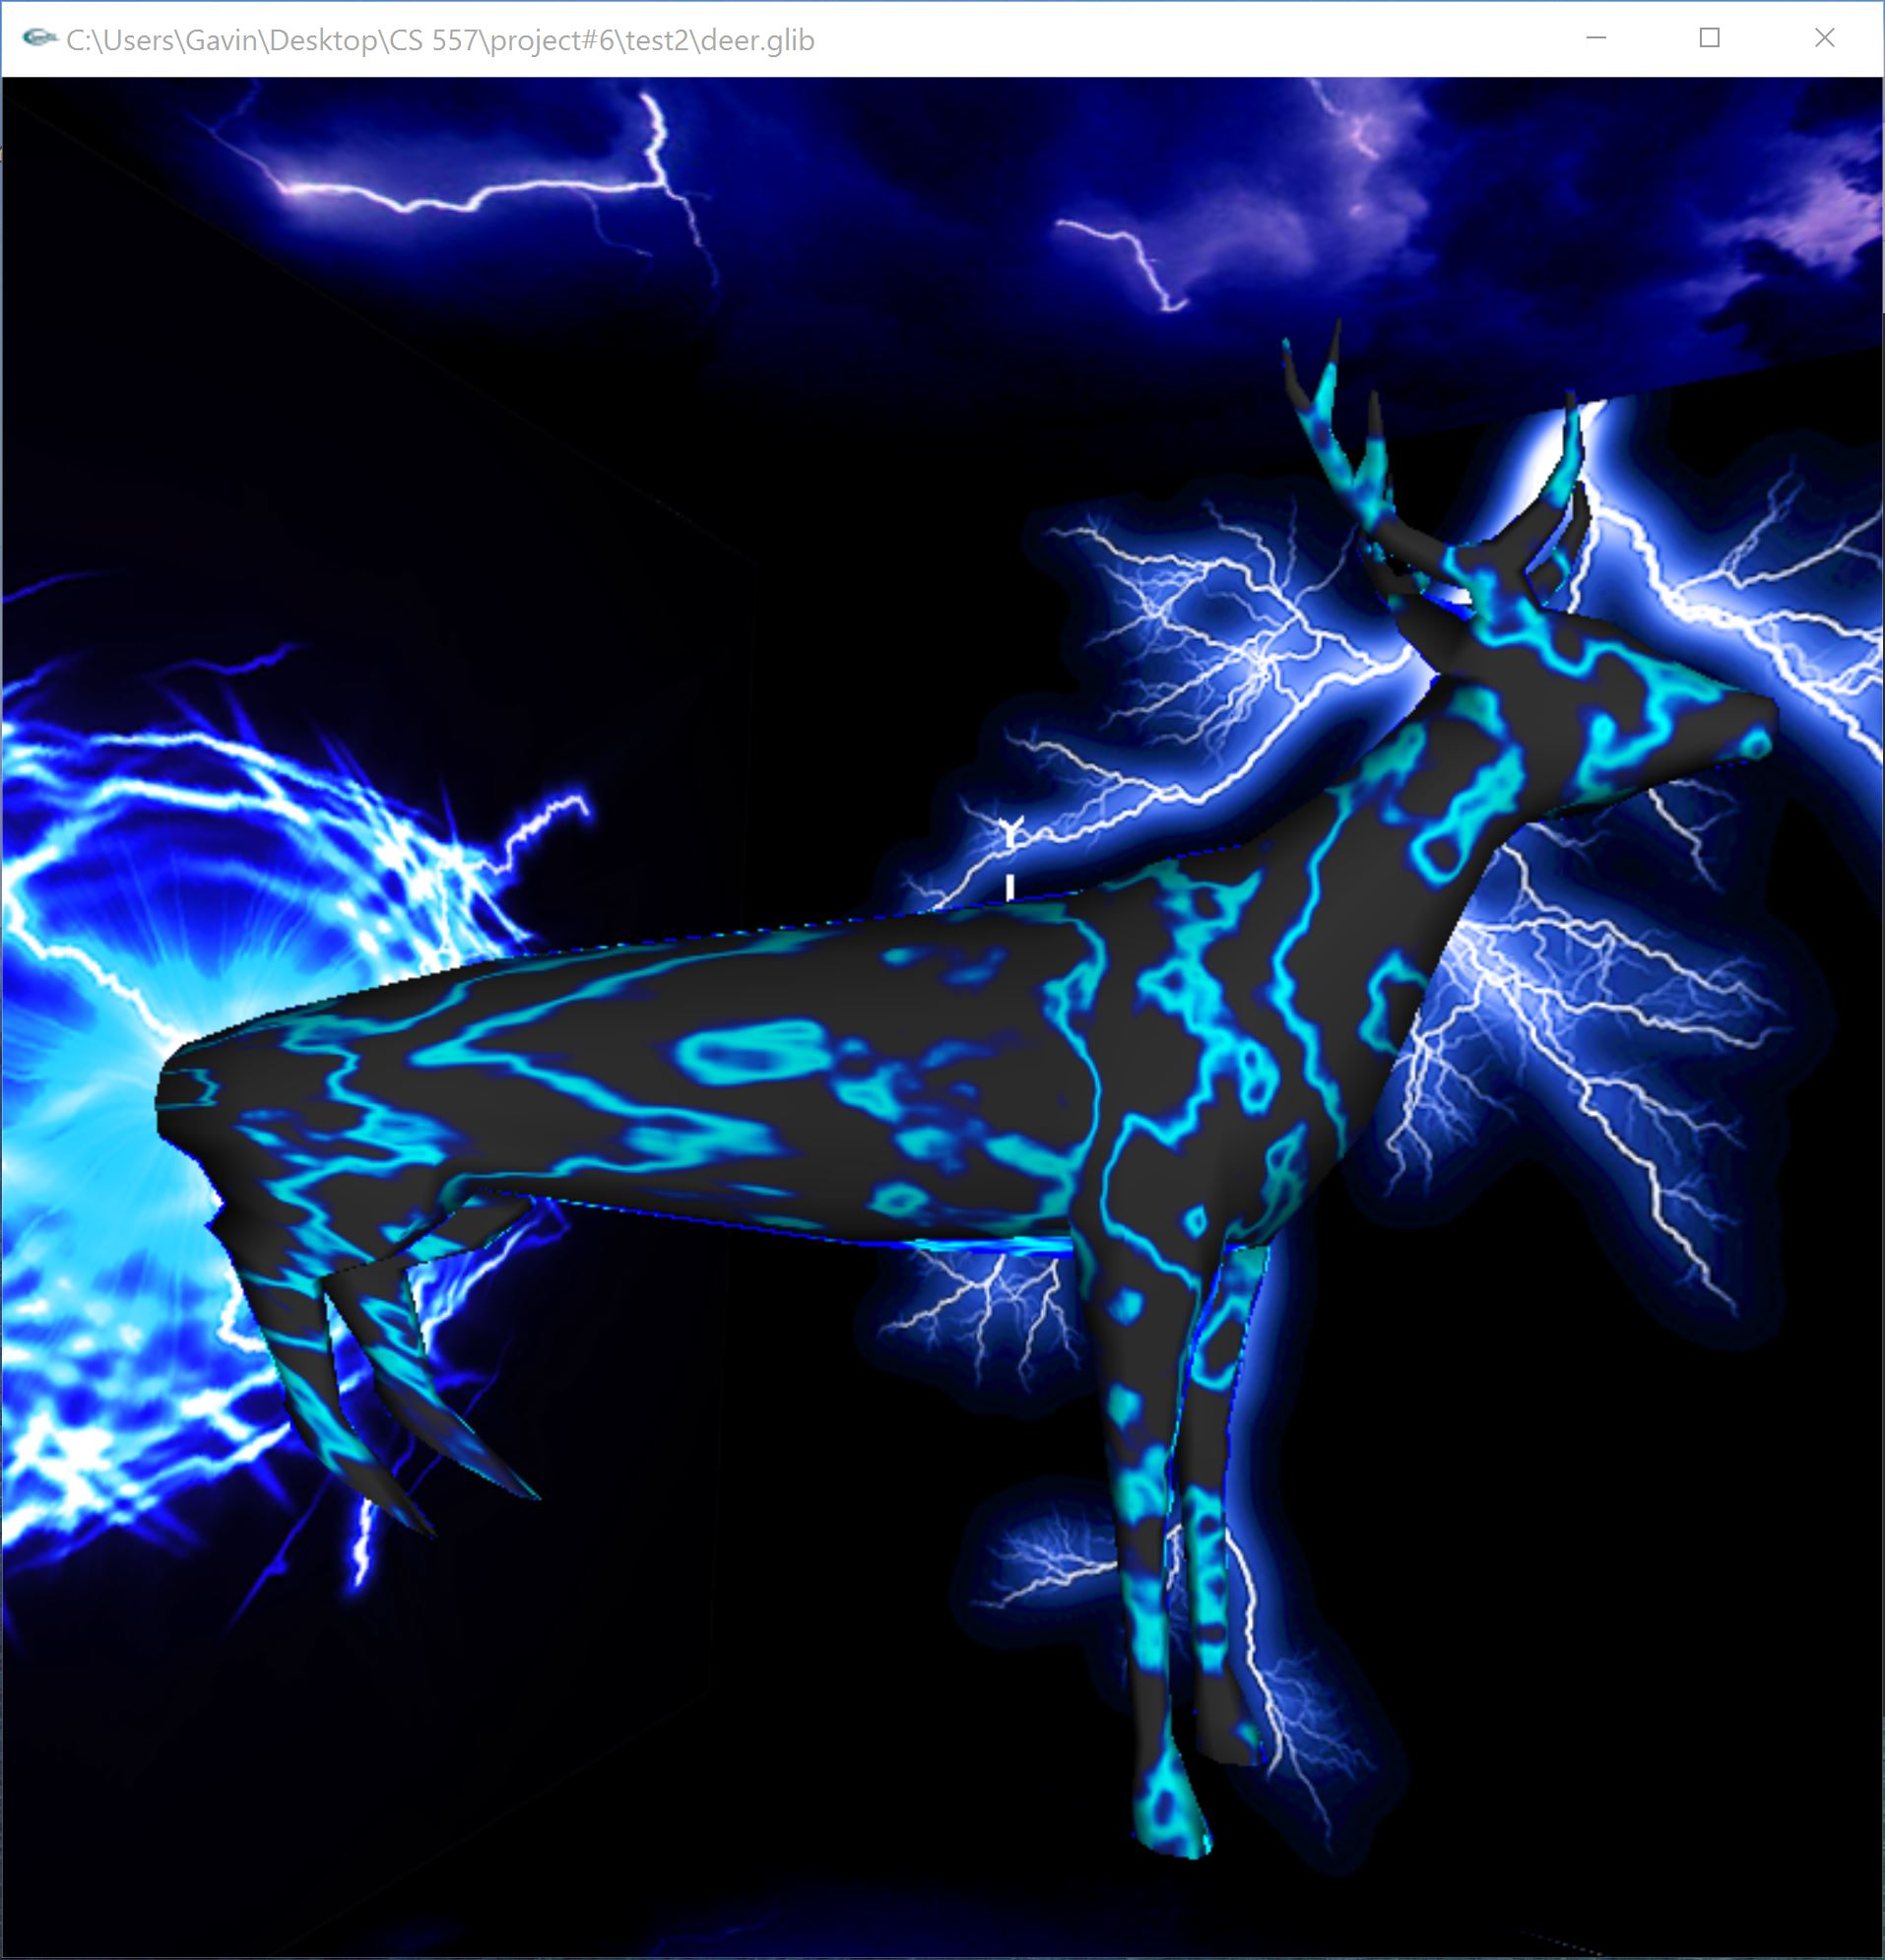
\includegraphics[width=2.8in]{noise.jpg}
 \end{center}
 The third part is adding fake silhouettes to the deer. I didn't use the geometry shaders to implement this, instead, I used a simpler way to do so. I checked every fragment's normal, and used it to calculate a dot product with the view direction. then I applied a threshold to limited the value in order to control the range of the area. The view direction is handled by the opposite direction of the eye coordinate vector. By controlling the threshold, I could change the ``silhouettes'' area on the deer's body. When dealing with the fragments in the area, I mixed the color with blue in order to implement a kind of lightning covering on the deer's body. The following image shows the effect, and it's pretty much like the poster.
 \begin{center}
 	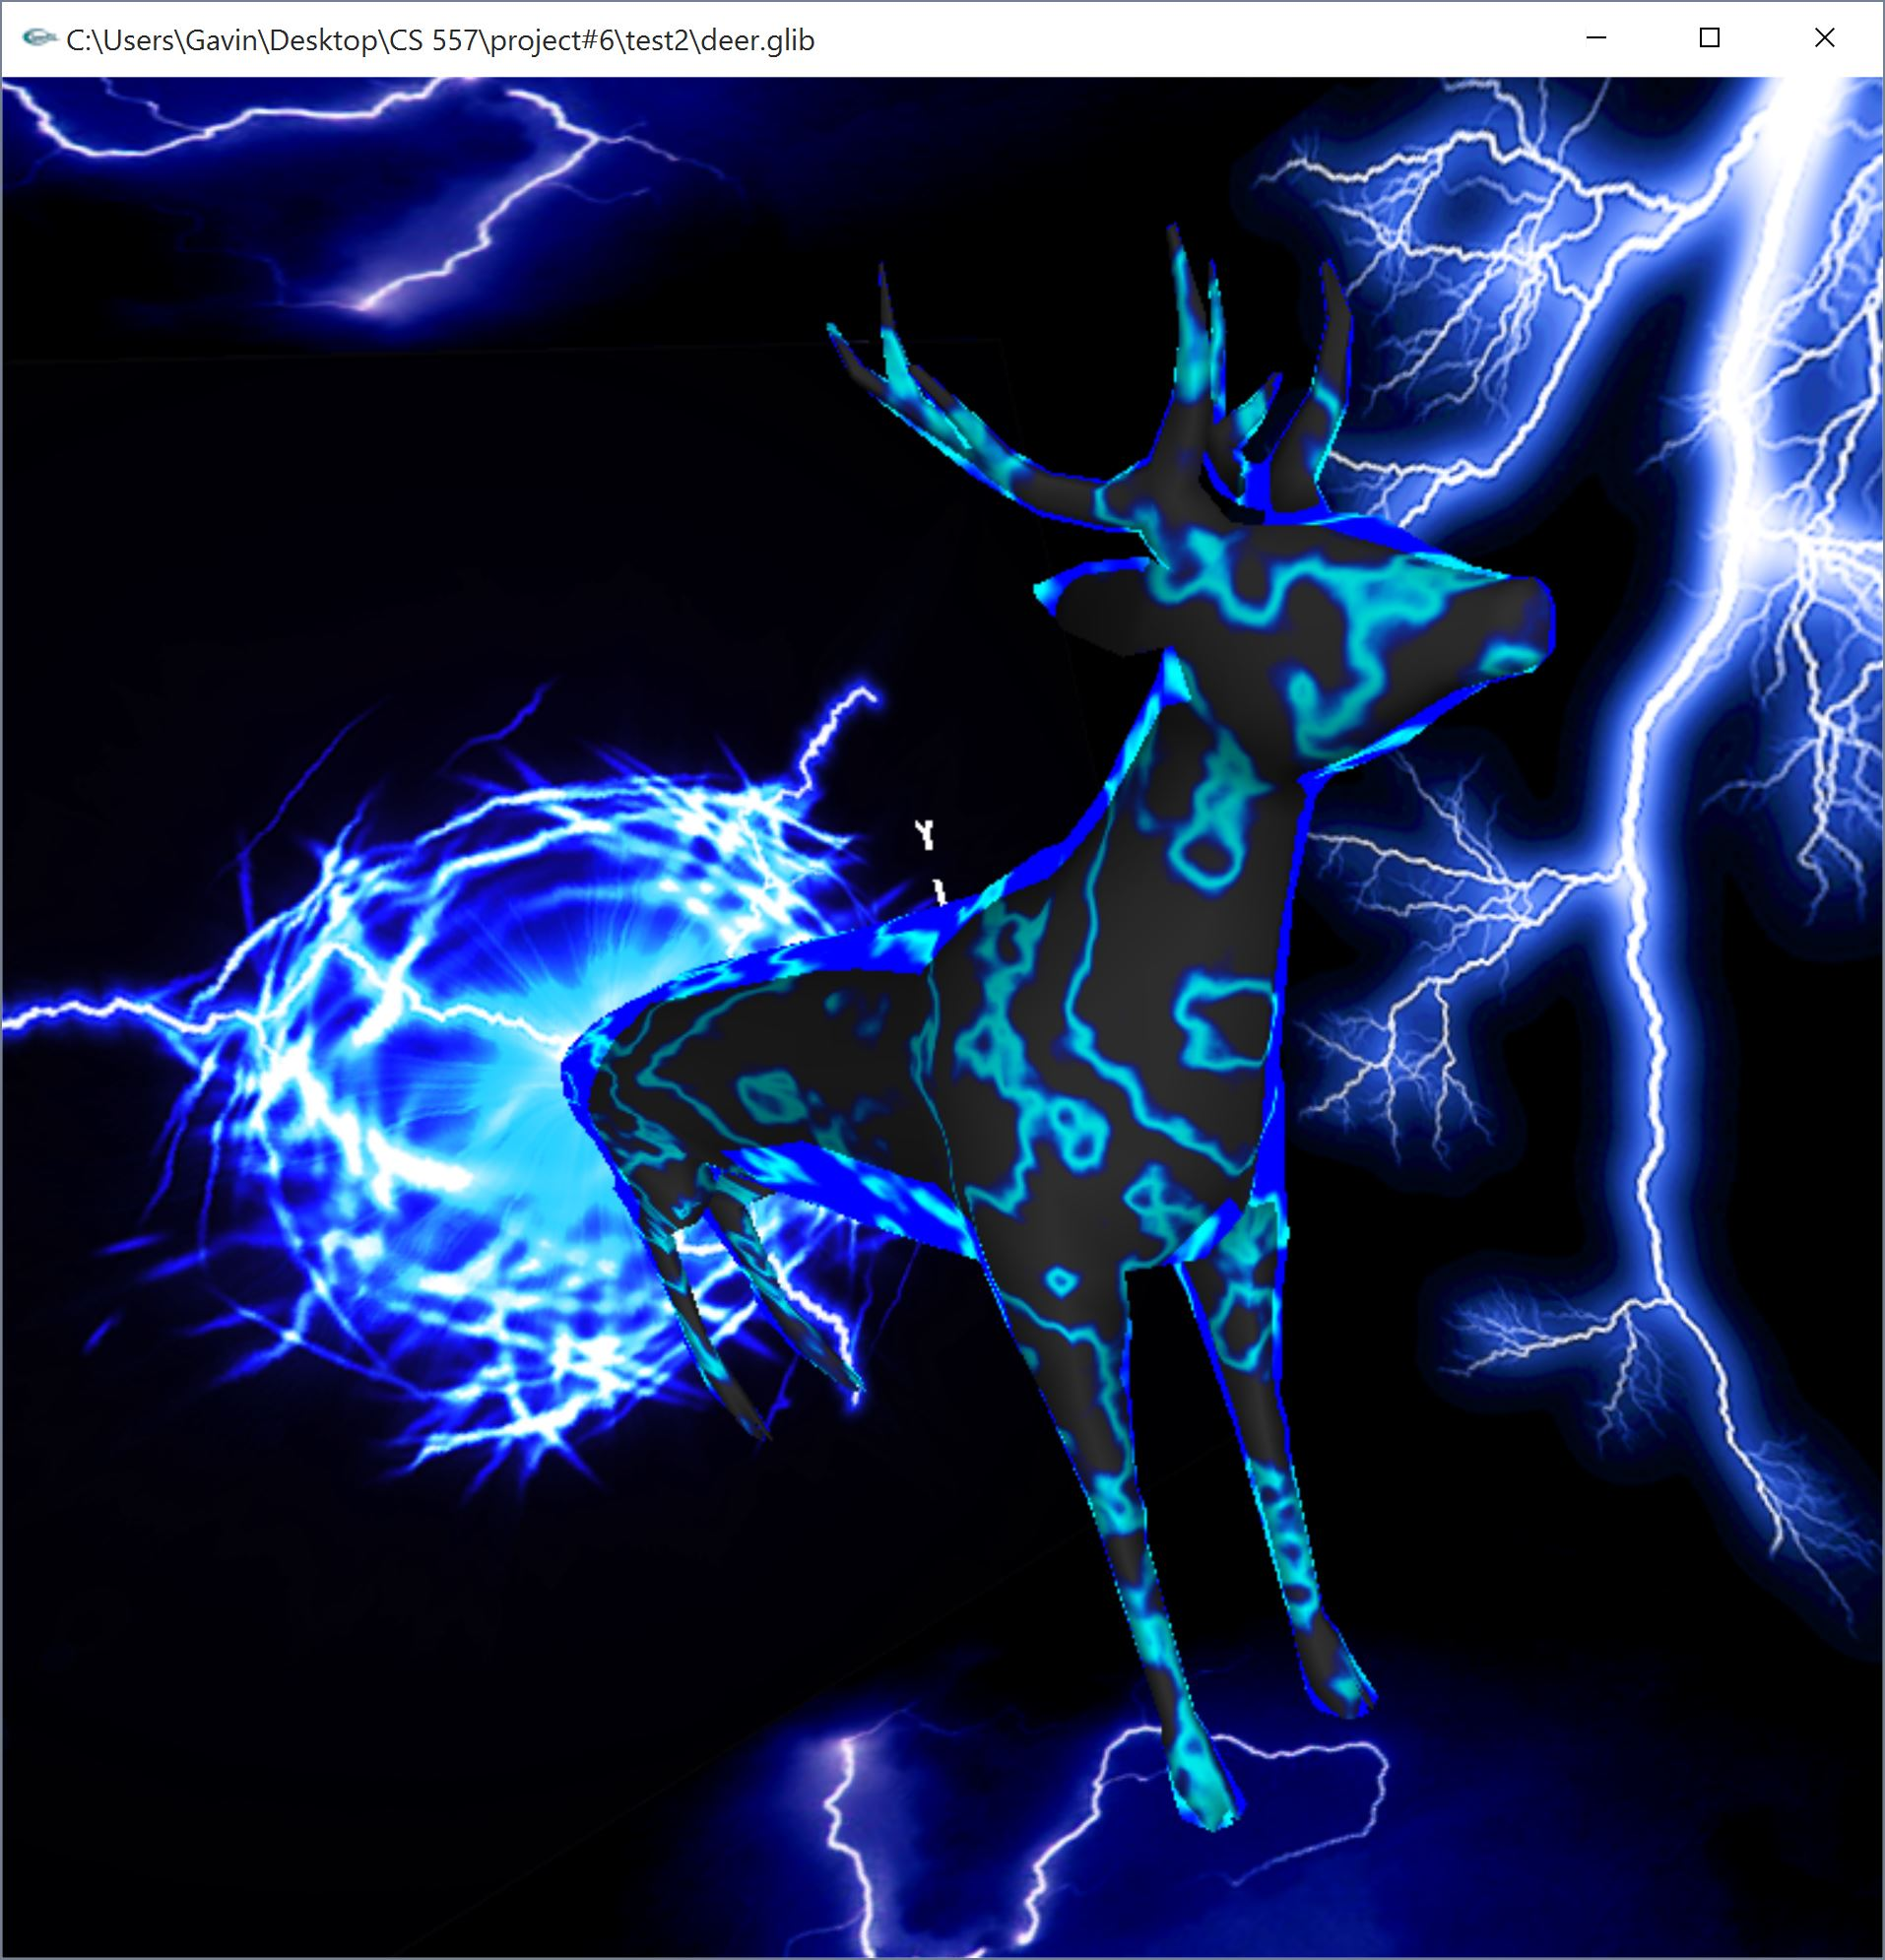
\includegraphics[width=3.2in]{silho.jpg}
 \end{center}
\section{Summary}
I think this project is kind of hard to do. The hard part is not about the real implementing but is about what to implement. I think the biggest limitation I had in this project is my imagination. I would like to create something not that easy to do and unique from what people did in the previous years. I changed my plan for several times and it resulted in the present one. All the techniques I used are what we have done in the previous class except the ``fake silhouettes'' and the ``silhouettes'' is also easy to do. I hope this poster could meet the ``Did it really well'' standard.
\end{document}